\section{Revising the Assumptions About Predictive Markets}
\label{sec:revising_assumptions}

\subsection{Efficency and Arbitrage opportunities}
\label{subsec:efficency_and_arbitrage_opportunities}

Predictive markets, such as Polymarket, should theoretically work well and be very efficient, so arbitrage opportunities would not be expected to be persistent \parencite{luckner2008arbitrage}. These are designed to be extremely efficient because they combine data from a wide range of participants, which results in the formation of prices that accurately reflect the likelihood of future events. This implies that market participants seeking to capitalize on these differences should quickly eliminate any price discrepancies that could create arbitrage opportunities.

However, it is essential to understand that no market can operate perfectly all the time. In practice, brief arbitrage opportunities may arise because information updates are delayed, market liquidity constraints are imposed, or market participants' responses to new information are delayed. Fast and agile arbitrageurs can exploit these opportunities, although rare and usually short-lived in efficient predictive markets.

Based on the data gathered by \cite{kapp2023improved} in their study on the accuracy of Polymarket, arbitrage opportunities appear to increase as the time frame for the occurrence of the event extends. This is because as the agreed-upon date for the event draws nearer, more information becomes available, and the predicted probability aligns more closely with the actual likelihood, eliminating arbitrage options. Additionally, these data reveal a clear relationship between arbitrage opportunities and the volume of contracts. Markets with a low volume of transactions, lacking a considerable number of agents, tend to be less efficient, and their prices often deviate more from the actual probability of the event, thus creating clear arbitrage opportunities. From the foregoing and the data available on Polymarket, we can assert that in mature markets with high agent participation, arbitrage opportunities tend to be nonexistent.

Because user bases and skill levels vary, so do market expectations and pricing, it is possible to explain the discrepancy in prices across various predictive markets. Furthermore, the efficiency of price adjustments is influenced by platform-specific variations in liquidity. Price disparities can also be caused by the dissemination and processing of information, transaction costs, and platform usability, as these factors can influence trader participation and market efficiency. These elements may contribute to the persistence of price disparities, particularly in more closed markets.

On the other hand, the presence of a potential arbitrage opportunity between predictive markets is observed, as seen in Image \ref{fig:market_comparison} obtained from \cite{Polack}, where the occurrence of a discovery in the superconductor sector is questioned. Although the question and criteria are the same, there is a discrepancy in the market price between the Metaculus, Manifold, and Polymarket platforms.

\begin{figure}[H]
    \centering
    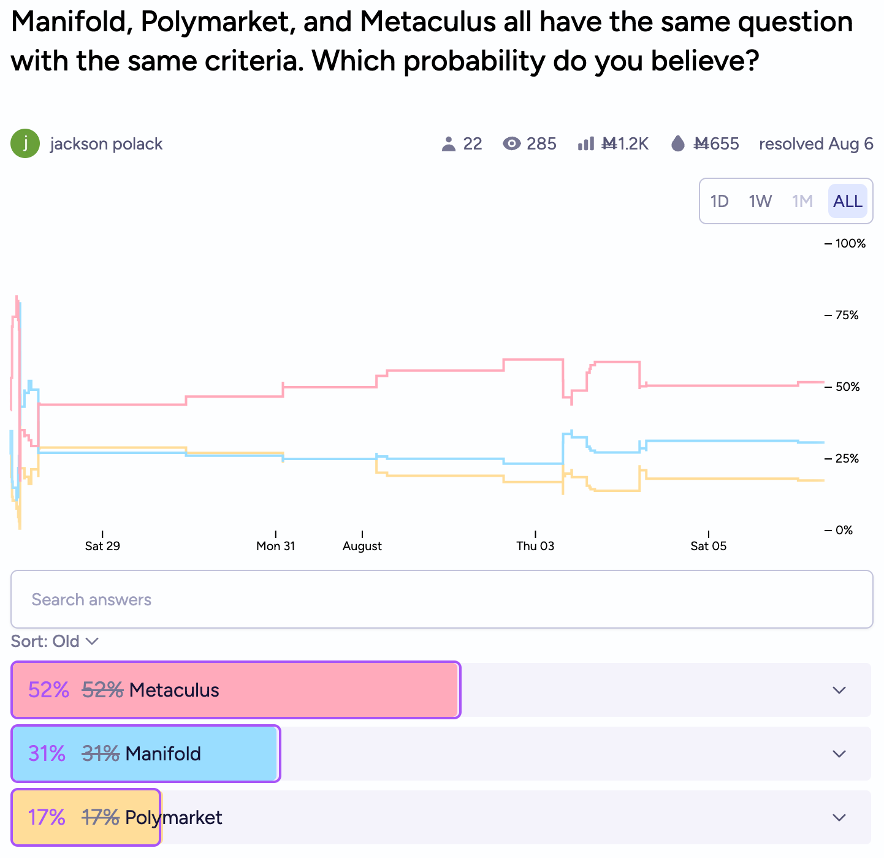
\includegraphics[scale=0.6]{img/MarketComparison.png}
    \caption{Comparison of the price of the same question in different predictive markets}
    \label{fig:market_comparison}
\end{figure}

This type of divergence is also common in cryptocurrencies predictive markets, because as the user bases and skill levels vary, so do market expectations and pricing. Furthermore, the efficiency of price adjustments is influenced by platform-specific variations in liquidity. Price disparities can also be caused by the dissemination and processing of information, transaction costs, and platform usability, as these factors can influence trader participation and market efficiency. These elements may contribute to the persistence of price disparities, particularly in more closed markets.

\subsection{Low Susceptibility to Manipulation}
\label{subsec:low_susceptibility_to_manipulation}

As defined by \cite{buckley2017effect}:
\begin{quote}
    \textit{A manipulation is an attempt by an individual or group of traders to affect the price of contracts being traded on a prediction market in a manner which contradicts their privately held information.}
\end{quote}
    
A prediction market can be manipulated when buyers of shares artificially inflate the demand for a false security regarding the fulfillment of a contract \parencite{choo2022manipulation}. If the results of such a predictive market are used to make policy decisions (exogenous manipulation), for example, the manipulating agents are willing to pay the cost that the deviation from the market prediction implies.
    
According to the literature on predictive markets, it is assumed that these are robust against manipulations. It is based on the argument that, if some agent tries to set a price that is not based on available information, another agent could take advantage of this deviation to make profits \parencite{buckley2017effect}.
    
According to \cite{HANSON2006449}, predictive markets can be subjected to experimentation, as a scenario with a defined set of information and incentives can be reproducible. When subjected to experimentation, studies confirm this hypothesis; however, one of the limitations in these experimental exercises is that participants may incur losses associated with manipulation exercises. This might be true in most predictive markets, but if the manipulating agents value the outcome of the manipulation more than the cost it implies, the hypothesis might not hold \parencite{deck2013affecting}.

In the study conducted by \citeauthor{HANSON2006449}, those agents who were incentivized to manipulate, set prices that were higher compared to those without incentives. However, in their experiment, this manipulation did not have a significant effect on equilibrium prices. Nevertheless, their results depends on the suspicion that the market is being manipulated, meaning that non-manipulating agents are aware of the possible attempt to manipulate and, therefore, correct their prices expectations.
    
On the other hand, \citeauthor{deck2013affecting} designs an experiment with two fundamental differences from that proposed by \Citeauthor{HANSON2006449}: \begin{enumerate*}[label=(\roman*)]
    \item the number of shares is not fixed, but any amount of shares can be bought or sold, and
    \item the manipulating agents have perfect information, and their profits do not depend on the number of shares they hold, but on the market outcome itself.
\end{enumerate*} 
The second point makes manipulators have the maximum incentive to intervene in the market. The conclusion of this study is that the presence of such manipulating agents makes the market unable to aggregate an accurate prediction. Additionally, in this study, it was determined that the manipulation strategy consists of increasing the volume of traded shares compared to the non-manipulated market, achieving this by emptying the Ask offers in the Order Book and, consequently, altering the equilibrium price.